\section{Cota inferior del anti-thickness geométrico de $K_n$}\label{sec:cota_inf}
El principal resultado de este trabajo es que encontramos el valor exacto del
anti-thickness geométrico para la gráfica completa de hasta diez vértices en
posición general. Obtuvimos dicho valor mejorando la cota inferior
(\ref{estado_atg_1}) y usando la cota superior actual mencionadas en el capítulo
\ref{cap3}. Empezamos explicando el proceso para encontrar la cota inferior.

Un conjunto de $n$ puntos en el plano induce una gráfica completa con $n$
vértices a la que denotamos como $K_n$. Como es completa $|E(K_n)|=
\binom{n}{2}$.
Cuando se quiere encontrar una descomposición de tamaño mínimo en thrackles una idea intuitiva es buscar que los thrackles tengan el mayor número posible de aristas. El siguiente teorema es útil para nosotros ya que establece el número máximo de aristas que puede tener un thrackle geométrico.
\begin{theorem}(\cite{Pach2013b})
  Toda gráfica geométrica de $n$ vértices en la
  que no existen dos aristas disjuntas tiene a lo más $n$ aristas. Esto se
  cumple para toda $n>2$.
\end{theorem}

Omitimos la demostración del teorema anterior ya que las ideas de la
demostración no son retomadas en este trabajo. El teorema es importante para
nosotros ya que indica el número máximo de aristas posibles para un thrackle.

Como mencionamos en el capítulo de antecedentes, un thrackle de $n$ vértices
con exactamente $n$ aristas es un thrackle máximo. Por definición, toda
descomposición de la gráfica completa cubre sus aristas. Si suponemos que
existen $k$ thrackles máximos en la descomposición, entonces la siguiente
desigualdad expresa el número de thrackles máximos necesarios para cubrir las
$\binom{n}{2}$ aristas de la gráfica completa:
\[ kn \geq \binom{n}{2}. \]

Como los thrackles de la descomposición son geométricos, si buscamos la $k$ más pequeña para la cual se cumple la desigualdad anterior entonces $k$ es el anti-thickness geométrico de la gráfica completa.
Resolviendo para $k$  tenemos que al menos
$k\geq\left\lceil\frac{n-1}{2}\right\rceil$ thrackles máximos son necesarios
para dar una descomposición de $K_n$. En otras palabras
\begin{equation}
  At_g(K_n) \geq  \left\lceil\frac{n-1}{2}\right\rceil.
  \label{resultados_cotainf_1}
\end{equation}

La tabla~\ref{table:attrivialinf} ilustra el valor de la cota inferior del
anti-thickness geométrico dada por (\ref{resultados_cotainf_1}) para $n\leq 10$.
\begin{table}[t]
  \centering
  \begin{tabular}{|c|c|}
    \hline
    $n$ & $\left\lceil\frac{n-1}{2}\right\rceil$ \\[5pt] \hline\hline
    3   & 1  \\
    4   & 2  \\
    5   & 2  \\
    6   & 3  \\
    7   & 3  \\
    8   & 4  \\
    9   & 4  \\
    10  & 5  \\ \hline
  \end{tabular}
  \caption{ Valor de la cota inferior del anti-thickness geométrico usando la cota trivial. }
  \label{table:attrivialinf}
\end{table}
Esta cota es la más inmediata ya que usa el hecho de que cada thrackle máximo tiene a lo sumo tantas aristas como vértices. También es la cota actual para el anti-thickness geométrico~(\cite{Dujmovic2017}).

En el trabajo de~\cite{Fabila-Monroy2018} encuentran que, dados dos thrackles
máximos en posición convexa, estos comparten una arista, y que esto se cumple
para cada par de thrackles de la descomposición. En este trabajo verificamos
que este resultado también es válido para conjuntos de hasta diez puntos en
posición general. Usando los tipos de orden de los conjuntos
con hasta diez puntos inducimos la gráfica completa, luego buscamos, para
cada uno de los tipos de orden, todos los thrackles máximos y
finalmente comparamos dichos thrackles a pares y encontramos que:
\begin{itemize}
  \item Cada par de thrackles máximos tienen intersección no vacía en aristas,
  para todo tipo de orden con al menos dos thrackles máximos.
  \item Existen tipos de orden con solo un thrackle máximo.
  \item Existen tipos de orden en los que no hay thrackles máximos.
\end{itemize}

Para buscar los thrackles máximos usamos el algoritmo~\ref{algo_kthrackles}
descrito en la sección~\ref{seccion_algoritmo_kthrackles}.Para comparar los
thrackles a pares utilizamos el algoritmo~\ref{algo_interseccion} descrito en
la misma sección. Describimos los algoritmos usados en otra sección para no
romper con el flujo matemático de esta sección. La lista de tipos de orden
con un solo thrackle máximo puede ser descargada de la siguiente liga:
\url{http://computacion.cs.cinvestav.mx/~dmerinos/site/archivos_tesis/withone_max.tar.gz}.
La lista de tipos de orden para los cuales no existe un thrackle máximo
está en la siguiente liga:
\url{http://computacion.cs.cinvestav.mx/~dmerinos/site/archivos_tesis/without_max.tar.gz}.

Gracias a estos resultados podemos derivar el siguiente lema.
\begin{lemma}\label{lema:thdisjuntos}
  Sea $S$ un conjunto de puntos en posición general y sean $T_1$ y $T_2$ thrakles máximos en $K_n(S)$ con $|V(T_1)|\leq 10$
  y $|V(T_2)|\leq 10$. $T_1$ y $T_2$ tienen al menos una arista en común.
\end{lemma}
\begin{proof}
  Para cada tipo de orden con hasta diez puntos, generamos todos los thrackles
  máximos inducidos. Usando este conjunto verificamos que para cada pareja la intersección en aristas es no vacía
\end{proof}
Esto implica que para $n\leq 10$ no es posible encontrar una descomposición
en thrackles máximos de tamaño $\left\lceil\frac{n-1}{2}\right\rceil$, ya que
los thrackles máximos no son disjuntos a pares y esto infringe las condiciones
de una descomposición.
Esto significa que una descomposición por thrackles solo podría contener un
thrackle máximo. Sin embargo, dada una colección de thrackles máximos, cuya
unión induce a $K_n$, es posible encontrar una colección de thrackles, no
necesariamente máximos, que son disjuntos en aristas y contar cuántas aristas
es posible cubrir con dicha colección. Describimos este proceso en el siguiente
lema:
% Por consecuencia es posible contar cuántas aristas son cubiertas
% por una descomposición de thrackles máximos cuyo tamaño es $\left\lceil\frac{n-1}{2}\right\rceil$.
\begin{lemma}\label{lema:existedescomp}
  Sea $\mathcal{C}=\{T_1,T_2,\cdots,T_m\}$ una colección de thrackles máximos
  de $K_n$ con $|E(T_i)\cap E(T_j)| = 1$.
  Existe una colección $\mathcal{D}$ de $K_n$ inducida por $\mathcal{C}$ donde
  para cada par de thrackles en $\mathcal{D}$ su intersección en aristas es
  vacía y cuyo número de aristas cubiertas es: \[\displaystyle \sum^n_{i=(n-m)
  + 1}i\].
\end{lemma}
\begin{proof}
  Sea $T'_i$, con $1 \leq i \leq m$ un thrackle inducido por el siguiente
  conjunto de aristas:
  \[\{E(T_i) - \bigcup_{k=1}^{i-1} E(T_i)\cap E(T_k)\} \}\]
  es decir $T'_i$ es el thrackle que tiene todas las aristas de $T_i$
  a excepción de aquellas que $T_i$ comparte con el resto de los thrackles
  en la colección.

  Sea $\mathcal{D}=\{T'_1,T'_2,\dots,T'_m\}$, por construcción, la intersección
  en aristas de cualesquiera dos thrackles de $\mathcal{D}$ es vacía.

  Nótese que si una arista $e$ aparece en dos thrackles de $\mathcal{C}$
  entonces, en $\mathcal{D}$, $e$ aparecerá únicamente en el thrackle con menor
  etiqueta.
  De hecho $T_1'$ tiene $n$ aristas, $T_2'$ tiene $n-1$ aristas, $T_3'$ tiene
  $n-2$ aristas y, en general, $T_i'$ tiene $n-i+1$ aristas. Como $\mathcal{D}$
  tiene $m$ thrackles el número de aristas cubiertas por $\mathcal{D}$ es
  \[ n + (n-1) + (n-2) + \cdots + (n-m) + (n - m + 1)\]
  Podemos escribir esta suma como :
  \[\displaystyle \sum^n_{i=(n-m) + 1}i\]
\end{proof}
% Ahora procedemos a contar el número de aristas que pueden ser cubiertas por una
% colección de thrackles disjuntos en aristas inducida por otra colección de
% thrackles máximos.
% \begin{lemma}\label{lema:numaristascubiertas}
%   Sea \[\mathcal{C}=\{T_1,T_2,\dots,T_m\}\] una colección de thrackles máximos.
%   y sea $\mathcal{D}$ la colección de thrackles disjuntos en aristas inducida
%   por $\mathcal{C}$.
%
%   El número de aristas cubiertas por $\mathcal{D}$ es exactamente :
%    \[\displaystyle \sum^n_{i=\left(n-m\right) + 1}i\]
%  \end{lemma}
%  \begin{proof}
%    Por construcción y por el lema~\ref{lema:thdisjuntos}: $T'_1$ tiene $n$
%    aristas, luego $T'_2$ tiene $n-1$
%    aristas, en general $T'_i$ tiene $n-(i-1) = n-i+1$ aristas. Como
%    $\mathcal{D}$ tiene $m$ thrackles el número de aristas cubiertas por
%    $\mathcal{D}$ es
%
%    Podemos escribir esta suma como:
%
%  \end{proof}
% Por consecuencia es posible contar cuántas aristas serán cubiertas si la descomposición es de thrackles
% máximos y tiene tamaño $\left\lceil\frac{n-1}{2}\right\rceil$ como sigue: el primer thrackle
% cubre $n$ aristas, el siguiente $n-1$ aristas, el próximo $n-2$ aristas
% y así sucesivamente tantas veces como thrackles tenga la descomposición, en este caso
% existen $\left\lceil\frac{n-1}{2}\right\rceil$ thrackles máximos en la descomposición.
%
% Entonces el número de aristas cubiertas es:
% \[\displaystyle \sum^n_{i=\left(n-\left\lceil\frac{n-1}{2}\right\rceil\right) + 1}i.\]
Es importante notar que este es el número más grande de aristas cubiertas por
una colección de thrackles disjuntos en aristas inducida por una colección de
thrackles máximos, esto es debido a que en el lema~\ref{lema:thdisjuntos}
consideramos que la intersección en aristas de dos thrackles máximos es de
tamaño 1. No es dificil observar que si la intersección es más grande entonces
el número de aristas cubiertas por la colección inducida es menor.

Con los lemas anteriores es posible probar que la cota inferior del
anti-thickness geométrico de $K_n$ no es justa para toda $n$. El siguiente
teorema establece esta afirmación.
\begin{theorem}\label{teo:cotainf}
Sea $\mathcal{D}=\{T'_1,T'_2,\dots,T'_{\left\lceil\frac{n-1}{2}\right\rceil}\}$
una colección thrackles disjuntos en aristas inducida por una colección de
$\left\lceil\frac{n-1}{2}\right\rceil$ thrackles máximos.
$\left\lceil\frac{n-1}{2}\right\rceil$ thrackles máximos no son
suficientes para inducir una colección que cubra las aristas de $K_n$ para toda
$3 \leq n \leq 10$.
\end{theorem}
\begin{proof}
  Para cada $3 \leq n \leq 10$ aplicamos el resultado del
  lema~\ref{lema:existedescomp} y encontramos que para $n=\{5,7,8,9,10\}$ no es
  posible cubrir las aristas de $K_n$ con una colección de
  $\left\lceil\frac{n-1}{2}\right\rceil$ thrackles disjuntos en aristas.
\end{proof}
En la tabla~\ref{table:attrivialtight} mostramos los casos para los que la cota
inferior del anti-thickness geométrico no es justa usando el
lema~\ref{lema:existedescomp}.
Es importante notar que este resultado es válido solamente cuando el dibujo de
$K_n$ tiene al menos
$\left\lceil\frac{n-1}{2}\right\rceil$ thrackles máximos.

\begin{table}[t]
  \centering
  \begin{tabular}{|c|c|c|c|}
    \hline
    $n$ & $\left\lceil\frac{n-1}{2}\right\rceil$ &
    $\sum^n_{i=\left(n-\left\lceil\frac{n-1}{2}\right\rceil\right) + 1}i$ &
    $\binom{n}{2}$\\[5pt] \hline\hline
    3   & 1  & 3 & 3 \\ \hline
    4   & 2  & 7 & 6 \\ \hline
    5   & 2  & \cellcolor{red!25}9 & 10 \\ \hline
    6   & 3  & 15 & 15 \\ \hline
    7   & 3  & \cellcolor{red!25}18 & 21 \\ \hline
    8   & 4  & \cellcolor{red!25}26 & 28 \\ \hline
    9   & 4  & \cellcolor{red!25}30 & 36 \\ \hline
    10  & 5  & \cellcolor{red!25}40 & 45 \\ \hline
  \end{tabular}
  \caption{ Mostramos cuántas aristas son cubiertas con una colección de
  $\left\lceil\frac{n-1}{2}\right\rceil$ thrackles máximos disjuntos en
  aristas. Se rellenan los casos en los que la colección no cubre todas las
  aristas. }
  \label{table:attrivialtight}
\end{table}

Como resultado del teorema~\ref{teo:cotainf} tenemos el siguiente corolario:
\begin{corollary}
  Para $n={5,7,8,9,10}$ no existe una descomposición de $K_n$ formada por
  $\left\lceil\frac{n-1}{2}\right\rceil$ thrackles máximos.
\end{corollary}

Gracias al lema~\ref{lema:existedescomp} y al teorema~\ref{teo:cotainf} podemos dar el valor exacto del número de thrackles máximos necesarios para inducir una descomposición por thrackles de $K_n$ con $ 3\leq n \leq 10$.

\begin{theorem}\label{teo:nuevacotainf}
  Si $\mathcal{D}$ es una colección de thrackles disjuntos en aristas inducida por una colección de $k$ thrackles máximos entonces :
  \[
    k = \left\{ \begin{array}{lr}
      \left\lceil\frac{n-1}{2}\right\rceil,     & \text{para } n\in\{3,4,6\}\\
    \left\lceil\frac{n-1}{2}\right\rceil + 1, & \text{para } n\in\{5,7,8,10\}\\
      \left\lceil\frac{n-1}{2}\right\rceil + 2, & \text{para } n=9
    \end{array} \right\}
  \]
\end{theorem}
\begin{proof}
  La prueba consiste en evaluar el número de aristas cubiertas por $k$
  thrackles usando el resultado del lema~\ref{lema:existedescomp}
  hasta encontrar $k$ suficientemente grande para que la descomposición
  cubra las $\binom{n}{2}$ aristas de $K_n$.
\end{proof}
Los resultados del teorema~\ref{teo:nuevacotainf} se presentan en la tabla~\ref{table:atnuevacota}.
\begin{table}[t]
  \centering
  \begin{tabular}{|c|c|c|c|}
    \hline
    $n$ & $k$ & $\sum^n_{i=(n-k) + 1}i$ & $\binom{n}{2}$\\[5pt] \hline\hline
    3   & 1  & 3 & 3 \\ \hline
    4   & 2  & 7 & 6 \\ \hline
    5   & 3  & 12 & 10 \\ \hline
    6   & 3  & 15 & 15 \\ \hline
    7   & 4  & 22 & 21 \\ \hline
    8   & 5  & 30 & 28 \\ \hline
    9   & 6  & 39 & 36 \\ \hline
    10  & 6  & 45 & 45 \\ \hline
  \end{tabular}
  \caption{Usando la cota del teorema~\ref{teo:nuevacotainf} para el número de
  thrackles máximos necesarios para inducir una descomposición es posible
  cubrir, para toda $n\leq 10$, las aristas de $K_n$.}
  \label{table:atnuevacota}
\end{table}

%

% Finalmente, usando el lema~\ref{lema:thdisjuntos} podemos ajustar la cota inferior.
%
% existe una descomposición de $k$ thrackles máximos entonces la descomposición
% cubre $kn - \binom{k}{2}$ aristas. Esto es exactamente igual que en el caso convexo.
% Podemos decir que para $n\leq 10$: \[ At_g(K_n) \geq  n - \Bigl\lfloor \sqrt{2n + \frac{1}{4}} - \frac{1}{2} \Bigr\rfloor. \]

% Podemos observar que esta cota inferior no es justa para toda $n\leq 10$. Por ejemplo
% si tomamos $n=5$, sabemos que la gráfica completa $K_5$ tiene $\binom{n}{2}=10$ aristas.
% Sabemos también que en $K_5$ los thrackles máximos tienen a lo sumo cinco aristas.
% Si es posible usar dos thrackles máximos para cubrir las diez aristas de $K_5$ significa que
% cada uno aporta exactamente cinco aristas y por lo tanto estos dos thrackles son disjuntos.
% Sin embargo nuestros resultados muestran que no existen dos thrackles máximos disjuntos
% para ningún dibujo de $K_5$. Entonces un thrackle máximo aporta cinco aristas y otro
% thrackle máximo aporta cuatro aristas, esto quiere decir que con dos thrackles máximos
% podemos cubrir nueve de las diez aristas de $K_5$, luego necesitamos un thrackle más
% para cubrir la arista restante. Decimos que el anti-thickness geométrico de $K_5$
% es al menos tres.

\section{Algoritmos}
En esta sección presentamos los algoritmos usados en el trabajo. Empezamos
describiendo el algoritmo para encontar thrackles de cualquier tamaño dado
un conjunto de puntos en posición general. Después hablamos del algoritmo
usado para encontrar la intersección de dos thrackles con el mismo número de
aristas. Luego...Finalmente...


\subsection{Algoritmo para encontrar thrackles con $k$
  aristas}\label{seccion_algoritmo_kthrackles}
  A continuación presentamos el algoritmo para encontrar thrackles de tamaño
  $k$. Para este algoritmo creamos una matriz con información de adyacencia a
  la que llamamos \emph{matriz de disyunción} (o \emph{disjointness matrix} en inglés).
  \begin{enumerate}
    \item Leer archivo de $n$ puntos para el tipo de orden deseado.
    \item Generar las aristas de la gráfica completa.
    \item Construir la matriz de disyunción.
    \item Obtener thrackles de tamaño $k$.
  \end{enumerate}

  El paso 2 consiste en generar y almacenar las $\binom{n}{2}$ combinaciones de
  pares de puntos leídos en el paso 1. En el paso 3 se construye una matriz
  cuadrada de $\binom{n}{2}$ filas, cada fila y cada columna representa una de
  las aristas de $K_n$. La matriz tiene un $0$ en la entrada $i,j$ si las
  aristas $i$ y $j$ se cruzan o comparten un vértice, de otra manera la entrada
  $i,j$ tiene un 1. En el paso 4 usamos la información de la matriz de
  disyunción previamente construida: Almacenamos un vector de enteros que tiene
  $k$ entradas dicho vector es inicializado con 0 en la primer entrada y 1 en
  la segunda entrada. Este vector representa un thrackle de tamaño $k$ que
  actualmente está compuesto por la arista 0 y cuyo tamaño se incrementará con
  el tiempo cuando se encuentre otra arista que también intersecte a la arista
  0. En general, supongamos que el vector actualmente tiene $i$ posiciones y
  deseamos saber si la arista $i+1$ puede formar parte del thrackle (con el
  objetivo de incrementar el tamaño del thrackle). Para ello, verificamos la
  intersección de la arista $i+1$ con las aristas del conjunto
  $\{0,1,2,\dots,i\}$. Puede ocurrir uno de dos casos :
  \begin{itemize}
    \item[a)] La arista $i+1$ no intersecta a alguno de las aristas en
    $\{0,1,2,\dots,i\}$. En este caso la arista $i+1$ no forma parte delel
    thrackle y debemos verificar con la siguiente arista, esta es, la arista
    $i+2$.
    \item[b)] La arista $i+1$ intersecta a todas las aristas en
    $\{0,1,2,\dots,i\}$. En este caso $i+1$ forma parte del thrackle y ahora el
    thrackle tiene $i+1$ aristas.
  \end{itemize}

  Repetimos esto hasta que el thrackle tenga $k$ aristas. Cuando el thrackle
  tiene $k$ aristas, almacenamos los valores del vector en una lista de
  vectores. Después, incrementamos el valor de la $k$-ésima entrada del vector
  en uno, si el valor nuevo es menor a $\binom{n}{2}$ la verificiación se hace
  como se describió antes.

  Si en algún momento la entrada $j$ del vector tiene un valor mayor o igual a
  $\binom{n}{2}$, esto es, que ya agotó los valores posibles para representar
  alguna arista en $K_n$, incrementamos el valor de la entrada $j-1$ y
  continuamos la verificación a partir de esta entrada como se describió
  anteriormente.

  El algoritmo descrito es un algoritmo de \emph{backtracking} que avanza
  mientras encuentre aristas que se intersecten a pares y regresa cuando se
  agotan las aristas posibles para incrementar el tamaño del thrackle. Debido a
  que los valores de las entradas del vector nunca se decrementan, el algoritmo
  agota los posibles valores para cada una de las entradas. Esto permite que
  regrese hasta la posición 0, cuando agote los $\binom{n}{2}$ valores para esta
  posición, intentará regresar a la posición -1 para continuar la verificación
  desde esa posición. Esta es una posición inválida para un vector, por ello
  usamos esta caracteristica como condición de paro de nuestro algoritmo.

  Los thrackles encontrados por este algoritmo están codificados como cademas de
  enteros, cada entero representa una de las aristas de $K_n$. Es posible
  inducir un thrackle a partir de un conjunto de aristas y después realizar
  operaciones sobre ellos.

  Debido a la construcción de la matriz de disyunción, y al algoritmo de
  backtracking, los thrackles encontrados están ordenados lexicograficamente. De
  tal manera que para el thrackle codificado como $i_1,i_2,\dots,i_k$ se tiene
  que $i_i < i_2 < \cdots < i_k$.

  El motivo por el que buscamos agotar las $\binom{n}{2}$ posibilidades para
  cada posición en el vector es que el algoritmo entrege todos los thrackles
  posibles con $k$ aristas.

  El pseudocódigo~\ref{algo_kthrackles} muestra el proceso del paso 4.
  \algblockdefx[NAME]{}{OTHEREND}%
  [1]{Until (#1)}
  \begin{algorithm}[htpb]
    \begin{algorithmic}[1]
      \Procedure{EncontrarThrackleK}{$n,k$}
      \State Sea $C$ un vector de tamaño $k+1$.
      \State $C[0]\gets 0$
      \State $C[1]\gets 1$
      \State \texttt{inters\_flag} $\gets$ \texttt{true}
      \State \texttt{curr\_size} $\gets 1$
      \While{$C[0] < \binom{n}{2}$}
      \While{\texttt{curr\_size}$<k$}
      \State \texttt{inters\_flag} $=$ \texttt{true}
      \If{$C[\text{\texttt{curr\_size}}] \geq \binom{n}{2}$}
        \State \texttt{curr\_size} $\gets$  \texttt{curr\_size} $-1$
        \If{\texttt{curr\_size} $<0$}
        \State \Return \texttt{thrackle\_counter}
        \EndIf
        \State $C[\text{\texttt{curr\_size}}]\gets C[\text{\texttt{curr\_size}}]+1$
        \State \textbf{continue}
      \EndIf
      \For{$i\gets 0 \dots \text{\texttt{curr\_size}}-1$}
        \State \texttt{inters\_flag}=\texttt{inters\_flag} $\&\&$ \texttt{matrix}$[C[i]][C\text{\texttt{curr\_size}}]$
      \EndFor
      \If{\texttt{inters\_flag} $==$ \texttt{False}}
        \State $C[\text{\texttt{curr\_size}}] \gets C[\text{\texttt{curr\_size}}] + 1$
      \Else
        \If{\texttt{curr\_size}$+1==k$}
          \State \texttt{thrackle\_counter} $\gets$ \texttt{thrackle\_counter} + 1
          \State Almacenar $C$ en una lista de vectores.
          \State \textbf{continue}
        \EndIf
      \EndIf
      \EndWhile
      \State $C[\text{\texttt{curr\_size}}+1] \gets C[\text{\texttt{curr\_size}}] + 1$
      \State \texttt{curr\_size} $\gets$ \texttt{curr\_size} $+1$
      \EndWhile
      \EndProcedure
    \end{algorithmic}
    \caption{Algoritmo para encontrar todos los thrackles de tamaño $k$.}
    \label{algo_kthrackles}
  \end{algorithm}

  La información de los thrackles encontrados para cada $3\leq n \leq 10$ es
  almacenada en archivos binarios de nombre \texttt{n\_k\_All\_bool.ths}
  donde \texttt{k} es el número de aristas para cada thrackle. El archivo binario
  tiene la siguiente estructura:
  \begin{enumerate}
    \item Tipo de orden escrito como caracter binario de tipo \texttt{uint16\_t}.
    \item Número de thrackles de tamaño $k$ para determinado tipo de orden
    escrito como caracter binario de tipo \texttt{uint16\_t}.
    \item Para cada thrackle, se escribe una lista de $\binom{n}{2}$ caracteres
    binarios que representan cada una de las aristas, si el $j$-ésimo elemento de
    la lista tiene un $0$ en el $i$-ésimo caracter entonces el thrackle $j$
    tiene la arista $i$. Cada caracter de la lista está escrito con un caracter
    de tipo \texttt{char}.
  \end{enumerate}

  La figura~\ref{fig:binaryfile} muestra un ejemplo de la sintaxis
  descrita anteriormente.
  \begin{figure}[htpb]
    \centering
    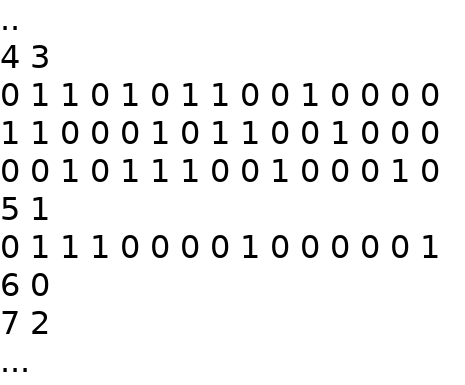
\includegraphics[width=0.4\linewidth]{binaryfile}
    \caption{Un segmento de un archivo binario, en este ejemplo $n=6$ y $k=6$.
    La primera línea indica que para el tipo de orden $4$ existen $3$ thrackles
    con $6$ aristas. Las siguientes 3 lineas indican las aristas de cada uno
    de los thrackles con un $1$. Después, para el tipo de orden 5, existe un
    thrackle, para el tipo de orden 6 no existen thrackles con 6 aristas. El
    archivo binario continua de esta manera para cada uno de los tipos de orden
    para $n=6$. Este ejemplo no representa necesariamente los datos reales
    encontrados en este trabajo para $n=6$.}
    \label{fig:binaryfile}
  \end{figure}

  Los datos de los thrackles máximos encontrados para cada $ 3\leq n \leq 9$
  pueden ser descargados de la siguiente liga:
  \url{http://computacion.cs.cinvestav.mx/~dmerinos/site/archivos_tesis/3to9.tar.gz}
  el archivo para $n=10$, separado debido a su tamaño,
   puede ser descargado de la siguiente liga:
  \url{http://computacion.cs.cinvestav.mx/~dmerinos/site/archivos_tesis/10.tar.gz}

\subsection{Intersección de dos thrackles}
  Dados dos thrackles con el mismo número de aristas, codificados como cadenas
  de enteros, aprovechamos el ordenamiento lexicográfico para hacer la
  operación de intersección de thrackles en tiempo lineal.
  Sea $A$ y $B$ dos vectores que representan las aristas de dos thrackles, con
  $|A|=|B|=k$. El algoritmo~\ref{algo_interseccion} entrega la intersección de $A$ y $B$ y la almacena en un conjunto $C$.
  \begin{algorithm}[htpb]
    \begin{algorithmic}[1]
      \Procedure{ThrackleIntersection}{$A,B,C$}
      \State $i\gets 0$
      \State $j\gets 0$
      \While{$i<k$ and $j<k$}
        \If{$A[i] < B[j]$}
          \State $i\gets i+1$
          \State \textbf{continue}
        \EndIf
        \If{$A[i]==B[j]$}
          \State $C\gets C\cup \{A[i]\}$
          \State $i\gets i+1$
          \State $j\gets j+1$
          \State \textbf{continue}
        \EndIf
        \If{$A[i]>B[j]$}
          \State $j\gets j+1$
          \State \textbf{continue}
        \EndIf
      \EndWhile
      \EndProcedure
    \end{algorithmic}
    \caption{Intersección de dos conjuntos ordenados en tiempo lineal.}
    \label{algo_interseccion}
  \end{algorithm}

\section{Descomposiciones por thrackles máximos.}

En este capítulo reportaremos el pseudocódigo de algoritmos usados durante el desarrollo
del proyecto así como los resultados que obtuvimos con dichos algoritmos.
Asímismo presentamos la prueba de que un thrackle que no es máximo no siempre
puede ser completado a uno máximo en posición general, mientras que en posición
convexa sí es posible.

% Inspirado en el método usado por~\cite{Fabila-Monroy2018} para posición convexa
% decidimos buscar para $n \leq 10$ descomposiciones de $K_n$ en la que los thrackles
% sean todos maximos y se alcance el anti-thickness establecido por el tipo de orden
% en posición convexa. Para esto buscamos para cada tipo de orden de cada $n \leq 10$
% todos los thrackles máximos y evaluamos cada combinación de tamaño $k_n$ con
% $k_n$ el anti-thickness convexo para conjuntos de tamaño $n$.
En el trabajo de~\cite{Fabila-Monroy2018} se encuentran descomposiciones de gráficas
geométricas en posición convexa usando thrackles máximos que comparten aristas a pares.
Usando esta idea y los datos de la tabla \ref{table:atconvexo} decidimos
buscar descomposiciones de $K_n$ para $n \leq 10$ en las que los thrackles
son todos máximos y cuyo tamaño sea el mismo del anti-thickness convexo para $K_n$.

\begin{table}[t]
  \centering
  \begin{tabular}{|c|c|}
    \hline
    $n$ & Anti-thickness convexo de $K_n$ ($At_c(n)$) \\ \hline\hline
    3   & 1  \\
    4   & 2  \\
    5   & 3  \\
    6   & 3  \\
    7   & 4  \\
    8   & 5  \\
    9   & 6  \\
    10  & 6  \\ \hline
  \end{tabular}
  \caption{ Anti-thickness convexo para $n\leq 10$ basado en el resultado de ~\cite{Fabila-Monroy2018}.}
  \label{table:atconvexo}
\end{table}

En resumen: para cada $n$ tomamos las combinaciones de $cat(n)$ thrackles máximos y
verificamos si alguna de estas combinaciones es una descomposición de $K_n$. Este proceso
lo repetimos para cada uno de los tipos de orden que hay para cada $n$.
Encontramos que sí existen tipos de orden que no corresponden al de posición convexa que también
alcanzan el anti-thickness convexo. Los resultados se muestran en la tabla \ref{table:res_desc_th_max}.
\begin{table}[t]
  \centering
  \begin{tabular}{|c|c|c|}
    \hline
    $n$   & Tipo de Orden & $k_n$ \\ \hline\hline
    8 & 12   & 5  \\
    8 & 54   & 5  \\ \hline
    9 & 12   & 6  \\
    9 & 52   & 6  \\
    9 & 54   & 6  \\
    9 & 80   & 6  \\
    9 & 696  & 6  \\
    9 & 1080 & 6  \\
    9 & 1287 & 6  \\ \hline
   10 & 81   & 6  \\
   10 & 1328 & 6  \\
   10 & 2243 & 6  \\ \hline
  \end{tabular}

  \caption{Tipos de orden para los que existe al menos una descomposición en thrackles máximos
  de tamaño igual al anti-thickness del tipo de orden convexo.}
  \label{table:res_desc_th_max}
\end{table}

Para los casos de $n \in \{3,4,\dots,7\}$ no pudimos encontrar una descomposición que cumpliera
con las caracteristicas antes descritas, esto es porque existen pocos tipos de orden
cuya unión de thrackles máximos cubran las aristas de la gráfica completa.
Los resultados fueron obtenidos con un algoritmo que primero evalúa
cuáles son los tipos de orden que podrían tener una descomposición por thrackles máximos;
se seleccionan aquellos que tengan suficientes thrackles máximos para cubrir todas las
aristas de la gráfica completa, en otras palabras que la unión de los thrackles
máximos en determinado tipo de orden cubran las $\binom{n}{2}$ aristas. Los pseudocódigos
de los algoritmos usados se encuentra en el algoritmo \ref{algo:maxthrackledecom} y
el algoritmo \ref{algo:finddecompositions}.

\begin{algorithm}[h!]
  \begin{algorithmic}[1]
    \Procedure{MaxThrackleDecom}{$n$}
    \State $vectorOT \gets \textit{valid-thrackles()}$
    \State $k \gets convexAt(n)$
    \ForEach {$ot \in vectorOT $}
        \State $n_{thr} \gets \textit{number of max thrackles on order type ot}$
        \State \textit{find-all-decomposition-of-size($n_{thr}$,k)}
    \EndFor
    \EndProcedure
  \end{algorithmic}
  \caption{Pseudocódigo del algoritmo que encuentra descomposiciones por thrackles
  máximos para todos los tipos de orden de una $n$ dada.}
  \label{algo:maxthrackledecom}
\end{algorithm}

\begin{algorithm}[h!]
  \begin{algorithmic}[1]
    \Procedure{find-all-decomposition-of-size}{$n_{thr},k$}
    \While{There is a combination $c$ of size $k$ from $\{0,1,\dots,n_{thr}\}$}
      \If{$c$ is a decomposition}
        \State visit $c$
      \EndIf
    \EndWhile
    \EndProcedure
    \caption{Pseudocódigo del algoritmo que encuentra combinaciones de $k$ thrackles
    máximos, si la combinación es una descomposición se visita.}
    \label{algo:finddecompositions}
  \end{algorithmic}
\end{algorithm}

Ejecutamos la implementación del algoritmo en el cluster:
para $n=8$ el resultado es obtenido en menos de un segundo mientras que para
$n=9$ y $n=10$ se necesitaron al rededor de 1 día y 6 días respectivamente.
Las decomposiciones encontradas pueden verse con más detalle en el apéndice XXXXX.

En el desarrollo del trabajo nos preguntamos por qué existen
otros tipos de orden diferente del convexo que tienen el mismo anti-thickness.
Algo en lo que pensamos fue en analizar de alguna manera la estructura de los
thrackles en dichos tipos de orden y por ello calculamos, para las descomposiciones
obtenidas mediante el método anteriormente descrito, el número de cruce de cada
uno de los thrackles de la descomposición. Se observa que en la mayoría de los
casos la mitad de los thrackles de las descomposiciones
tienen el número de cruce mínimo para $n$ vértices y la otra mitad es más
cercano al mayor número de cruce para $n$ vértices. Estos resultados pueden
estudiarse con más detalle een el apéndice XXXXXX.

\section{Anti-thickness geométrico exacto de $K_n$ con $3\leq n \leq 9$.}
\chaptermark{$gat(n)$ exacto para $3\leq n \leq 9$.}
Dado que la cota superior está dada por el anti-thickness convexo decidimos tratar
de ajustar la cota inferior ya que creemos que el anti-thickness geométrico es igual
al anti-thickness convexo. Un enfoque para ajustar la cota inferior es obtener el
anti-thickness de cada dibujo de $K_n$, esto es, obtener el anti-thickness de cada
tipo de orden para $K_n$ y seleccionar el menor de todos. Sin embargo, el algoritmo
exhaustivo para encontrar el anti-thickness tarda al rededor de 7 horas para un solo
tipo de orden cuando $n=8$, si para $n=8$ hay 3315 tipos de orden requeririamos
cerca de 960 días para acabar dicha tarea.

Por esta razón decidimos analizar la estructura de las posibles descomposiciones;
como $K_n$ tiene $\binom{n}{2}$ aristas y los thrackles de la descomposición deben
cubrirlas todas podemos buscar particiones de enteros de la forma $a_1 + a_2 + \dots +
a_k = \binom{n}{2}$.

A manera de ejemplo, mostraremos como se ajusta la cota inferior del anti-thickness
geométrico para $K_5$. En $K_5$ existen 10 aristas. Las siguientes son
particiones del entero 10:
\[
\begin{array}{l l}
  1 + 1 + 1 + 1 + 1 + 1 + 1 + 1 + 1 + 1 & 2 + 1 + 1 + 1 + 1 + 1 + 1 + 1 + 1\\
  3 + 1 + 1 + 1 + 1 + 1 + 1 + 1         & 2 + 2 + 1 + 1 + 1 + 1 + 1 + 1    \\
  4 + 1 + 1 + 1 + 1 + 1 + 1             & 3 + 2 + 1 + 1 + 1 + 1 + 1        \\
  2 + 2 + 2 + 1 + 1 + 1 + 1             & 5 + 1 + 1 + 1 + 1 + 1            \\
  4 + 2 + 1 + 1 + 1 + 1                 & 3 + 3 + 1 + 1 + 1 + 1            \\
  3 + 2 + 2 + 1 + 1 + 1                 & 2 + 2 + 2 + 2 + 1 + 1            \\
  6 + 1 + 1 + 1 + 1                     & 5 + 2 + 1 + 1 + 1                \\
  4 + 3 + 1 + 1 + 1                     & 4 + 2 + 2 + 1 + 1                \\
  3 + 3 + 2 + 1 + 1                     & 3 + 2 + 2 + 2 + 1                \\
  2 + 2 + 2 + 2 + 2                     & 7 + 1 + 1 + 1                    \\
  6 + 2 + 1 + 1                         & 5 + 3 + 1 + 1                    \\
  5 + 2 + 2 + 1                         & 4 + 4 + 1 + 1                    \\
  4 + 3 + 2 + 1                         & 4 + 2 + 2 + 2                    \\
  3 + 3 + 3 + 1                         & 3 + 3 + 2 + 2                    \\
  8 + 1 + 1                             & 7 + 2 + 1                        \\
  6 + 3 + 1                             & 6 + 2 + 2                        \\
  5 + 4 + 1                             & 5 + 3 + 2                        \\
  4 + 4 + 2                             & 4 + 3 + 3                        \\
  9 + 1                                 & 8 + 2                            \\
  7 + 3                                 & 6 + 4                            \\
  5 + 5
\end{array}
\]
Ahora bien, algunas de estas particiones pueden ser usadas como guía para encontrar
una descomposición en thrackles para $K_5$. Si tomamos, por ejemplo, la partición $5+4+1$
estaríamos buscando una descomposición por 3 thrackles: uno de tamaño 5, uno de tamaño 4
y otro de tamaño 1. Es importante notar que como las particiones de un entero $k$
suman exactamente $k$, los thrackles de la descomposición tienen que ser disjuntos en aristas
cuando los tamaños corresponden a los enteros de la partición de $k$.
La partición $5+4+1$ podría ser posible de encontrar, sin embargo, podemos
deshacernos de ciertas particiones que estamos seguros jamás encontraremos como son
aquellas particiones que tienen un entero mayor a $5$ puesto que para un conjunto
de $5$ vértices el thrackle geométrico más grande tiene $5$ aristas, esto también se cumple
para todo $n$. Desaparecerían entonces particiones como $7+2+1$ o $9+1$ por mencionar algunas.

Nuestro conjunto de particiones posibles se ve ahora de la siguiente manera:
\[
\begin{array}{l l}
  1 + 1 + 1 + 1 + 1 + 1 + 1 + 1 + 1 + 1 & 2 + 1 + 1 + 1 + 1 + 1 + 1 + 1 + 1\\
  3 + 1 + 1 + 1 + 1 + 1 + 1 + 1         & 2 + 2 + 1 + 1 + 1 + 1 + 1 + 1    \\
  4 + 1 + 1 + 1 + 1 + 1 + 1             & 3 + 2 + 1 + 1 + 1 + 1 + 1        \\
  2 + 2 + 2 + 1 + 1 + 1 + 1             & 5 + 1 + 1 + 1 + 1 + 1            \\
  4 + 2 + 1 + 1 + 1 + 1                 & 3 + 3 + 1 + 1 + 1 + 1            \\
  3 + 2 + 2 + 1 + 1 + 1                 & 2 + 2 + 2 + 2 + 1 + 1            \\
  5 + 2 + 1 + 1 + 1                     & 4 + 3 + 1 + 1 + 1                \\
  4 + 2 + 2 + 1 + 1                     & 3 + 3 + 2 + 1 + 1                \\
  3 + 2 + 2 + 2 + 1                     & 2 + 2 + 2 + 2 + 2                \\
  5 + 3 + 1 + 1                         & 5 + 2 + 2 + 1                    \\
  4 + 3 + 2 + 1                         & 4 + 4 + 1 + 1                    \\
  3 + 3 + 3 + 1                         & 4 + 2 + 2 + 2                    \\
  5 + 4 + 1                             & 3 + 3 + 2 + 2                    \\
  4 + 4 + 2                             & 5 + 3 + 2                        \\
  5 + 5                                 & 4 + 3 + 3
\end{array}
\]

Sin embargo, como buscamos ajustar la cota inferior del anti-thickness no nos
interesa encontrar descomposiciones cuyo tamaño sea mayor a la cota superior
del anti-thickness dada por $n - \lfloor \sqrt{2n + 1/4} - 1/2 \rfloor$, en el
caso de $n=5$, evitaremos buscar descomposiciones con un tamaño mayor a 3. Dejando
así las siguientes particiones disponibles:
\[
\begin{array}{l l}
  5 + 4 + 1                 & 4 + 4 + 2                                 \\
  4 + 3 + 3                 & 5 + 3 + 2                                 \\
  5 + 5
\end{array}
\]

Finalmente, vamos a remover las particiones cuyo tamaño sea igual al anti-thickness
convexo de $K_5$, esto porque sabemos que en efecto la posición convexa otorga
descomposiciones de ese tamaño. Esto nos deja con una única partición posible :
\[ 5 + 5 \] Esto significa que debemos averiguar si existe una descomposición
de $K_5$ por dos thrackles de tamaño 5, en este caso dos thrackles máximos. No obstante,
al buscar las thrackles máximos para todos los tipos de orden de $K_5$ encontramos
que no existen dos thrackles máximos que sean disjuntos en aristas, por esto no
es posible dar una descomposición de $K_5$ en dos thrackles máximos. Y luego,
el anti-thickness de $K_5$ es mayor a 2. Como la cota superior del anti-thickness
de $K_5$ es 3 podemos decir que el anti-thickness geométrico de $K_5$ es exactamente 3.

De esta manera podemos acotar el anti-thickness geométrico de $K_n$: examinar particiones
del entero $\binom{n}{2}$ con las siguientes condiciones:
\begin{itemize}
  \item La longitud de la partición es menor que el anti-thickness convexo de $K_n$.
  \item Solo existe una ocurrencia del entero $n$ en la partición.
\end{itemize}

Siguiendo las condiciones anteriores buscamos las particiones válidas para $K_n$
con $n\in[3,9]$. Encontramos que para $n\in[3,7]$ no existen particiones que
cumplan las condiciones, por lo que podemos decir que el anti-thickness geométrico
de $K_n$ para $n\in[3,7]$ es igual al anti-thickness convexo.

Para $K_8$ encontramos las siguientes particiones válidas:

\[
\begin{array}{l l}
8 + 7 + 7 + 6 & 7 + 7 + 7 + 7
\end{array}
\]

No fue posible encontrar una descomposición en thrackles usando alguna de estas
particiones, por lo que podemos decir que $K_8$ tiene anti-thickness geométrico
mayor a 4 y luego el anti-thickness geométrico de $K_8$ es exactamente 5.

Por otro lado para ajustar la cota inferior del anti-thickness de $K_9$,
tenemos las siguientes particiones válidas:
\[
\begin{array}{l l}
9 + 8 + 8 + 8 + 3 & 9 + 8 + 8 + 7 + 4 \\
9 + 8 + 8 + 6 + 5 & 9 + 8 + 7 + 7 + 5 \\
9 + 8 + 7 + 6 + 6 & 9 + 7 + 7 + 7 + 6 \\
8 + 8 + 8 + 8 + 4 & 8 + 8 + 8 + 7 + 5 \\
8 + 8 + 8 + 6 + 6 & 8 + 8 + 7 + 7 + 6 \\
8 + 7 + 7 + 7 + 7
\end{array}
\]

Para cada una de las particiones se diseñó un algoritmo que evalúa todos los thrackles
de tamaño 9, 8, 7 y 6. Los resultados fueron los siguientes:

\begin{itemize}
  \item 9 + 8 + 8 + 8 + 3 - Probado con 9+8+8.
  \item 9 + 8 + 8 + 7 + 4 - Probado con 9+8+8.
  \item 9 + 8 + 8 + 6 + 5 - Probado con 9+8+8. 150000ms
  \item 9 + 8 + 7 + 7 + 5 - Probado con 9+8+7+6+6
  \item 9 + 8 + 7 + 6 + 6 - Probado con 9+8+7+6+6. 981709 ms.
  \item 9 + 7 + 7 + 7 + 6 - Probado con 9+7+7+7+6. 2.11354e+06 ms.
  \item 8 + 8 + 8 + 8 + 4 - Probado con 8+8+8+8. 300888 ms.
  \item 8 + 8 + 8 + 7 + 5 - Probado con 8+8+8+6+6.
  \item 8 + 8 + 8 + 6 + 6 - Probado con 8+8+8+6+6. 569735 ms.
  \item 8 + 8 + 7 + 7 + 6 - Probado con 8+8+7+7+6. 6.39485e+06 - 1 Hora, 46 minutos.
  \item 8 + 7 + 7 + 7 + 7 - Probado con 8+7+7+7+7. 1.23716e+08 - 34 Horas, 21 minutos.
\end{itemize}

En la mayoría de los casos no fue necesario examinar toda la partición, por ejemplo
para la partición $9+8+8+8+3$, encontramos que no hay 3 thrackles, para ningún
tipo de orden diferente del convexo, donde uno sea de tamaño 9
y los otros dos de tamaño 8 que sean disjuntos en aristas y por esta razón no es necesario
seguir examinando la partición a fondo.

Como para ninguna partición fue posible encontrar una descomposición en thrackles
podemos decir que el anti-thickness geométrico de $K_9$ es mayor a 5. Y como la cota
superior del anti-thickness geométrico es 6 decimos que el anti-thickness de $K_9$
es exactamente 6.
